\textcolor{red}{We now report and discuss the main results of our longitudinal study of topic classification on Twitter, considering both the classification performance and our interpretation of which features are valuable in classification.}


\begin{table*}[t!]
\centering
\caption{Performance of topical classifier learning algorithms across metrics and topics with the mean performance over all topics shown in the right column. The best performance per metric is shown in bold.} 
{\def\arraystretch{1.2}
\resizebox{\textwidth}{!}{%
% Preview source code for paragraph 0

\begin{tabular}{|c|c|c|c|c|c|c|c|c|c|c|c|c|}
\hline 
\multicolumn{2}{|c|}{} & \multirow{2}{*}{\textbf{Tennis}} & \multirow{2}{*}{\textbf{Space}} & \multirow{2}{*}{\textbf{Soccer}} & \multirow{2}{*}{\textbf{Iran Deal}} & \textbf{Human} & \textbf{Celebrity} & \textbf{Social} & \textbf{Natural} & \multirow{2}{*}{\textbf{Epidemics}} & \multirow{2}{*}{\textbf{LGBT}} & \multirow{2}{*}{\textbf{Mean}}\tabularnewline
\multicolumn{2}{|c|}{} &  &  &  &  & \textbf{Disaster} & \textbf{Death} & \textbf{Issues} & \textbf{Disaster} &  &  & \tabularnewline
\hline 
\hline 
\textbf{LR} & \textbf{AP} & \textbf{0.9590} & 0.6452 & 0.5036 & \textbf{0.9807} & \textbf{0.6952} & 0.9293 & 0.5698 & \textbf{0.9428} & 0.4005 & 0.1559 & 0.6782$\pm$0.1724\tabularnewline
\hline 
\textbf{NB} & \textbf{AP} & 0.5859 & 0.8471 & 0.3059 & 0.9584 & 0.4224 & 0.4658 & 0.5030 & 0.3518 & 0.4050 & 0.1689 & 0.5014$\pm$0.1494\tabularnewline
\hline 
\textbf{RankSVM} & \textbf{AP} & 0.702 & 0.840 & \textbf{0.674} & 0.586 & 0.603 & 0.469 & 0.370 & 0.248 & 0.136 & 0.082 & 0.471$\pm$0.18\tabularnewline
\hline 
\textbf{RF} & \textbf{AP} & 0.9344 & \textbf{0.9314} & 0.5509 & 0.9757 & 0.6658 & \textbf{0.9571} & \textbf{0.8213} & 0.8306 & \textbf{0.5154} & \textbf{0.2633} & \textbf{0.7445$\pm$0.14764}\tabularnewline
\hline 
\textbf{KNN} & \textbf{AP} & 0.9550 & 0.7751 & 0.4739 & 0.9752 & 0.598 & 0.542 & 0.5078 & 0.9599 & 0.5317 & 0.1774 & 0.6496$\pm$0.1618\tabularnewline
\hline 
\hline 
\textbf{LR} & \textbf{P@10} & \textbf{1.0} & 0.2 & 0.3 & \textbf{1.0} & 0.5 & 0.8 & 0.2 & \textbf{1.0} & 0.5 & \textbf{0.6} & 0.61$\pm$0.2012\tabularnewline
\hline 
\textbf{NB} & \textbf{P@10} & 0.1 & \textbf{0.8} & 0.0 & 0.9 & 0.7 & 0.1 & 0.0 & 0.3 & 0.1 & 0.0 & 0.3$\pm$0.2225\tabularnewline
\hline 
\textbf{RankSVM} & \textbf{P@10} & \textbf{1.0} & \textbf{0.8} & \textbf{0.6} & 0.8 & 0.4 & 0.3 & 0.0 & 0.1 & 0.0 & 0.2 & 0.42$\pm$0.26\tabularnewline
\hline 
\textbf{RF} & \textbf{P@10} & \textbf{1.0} & 0.5 & 0.5 & \textbf{1.0} & \textbf{0.9} & \textbf{1.0} & \textbf{1.0} & \textbf{1.0} & \textbf{0.7} & 0.5 & \textbf{0.81$\pm$0.1444}\tabularnewline
\hline 
\textbf{KNN} & \textbf{P@10} & \textbf{1.0} & 0.0 & 1.0 & \textbf{1.0} & 0.7 & 0.9 & 0.0 & 0.9 & 0.3 & 0.4 & 0.62$\pm$0.2543\tabularnewline
\hline 
\hline 
\textbf{LR} & \textbf{P@100} & \textbf{0.98} & 0.65 & \textbf{0.44} & \textbf{0.99} & 0.74 & 0.94 & 0.59 & \textbf{0.98} & 0.45 & 0.2 & 0.696$\pm$0.1721\tabularnewline
\hline 
\textbf{NB} & \textbf{P@100} & 0.56 & \textbf{0.95} & 0.0 & 0.98 & 0.39 & 0.36 & 0.16 & 0.37 & 0.48 & 0.1 & 0.435$\pm$0.2033\tabularnewline
\hline 
\textbf{RankSVM} & \textbf{P@100} & 0.73 & 0.72 & 0.31 & 0.70 & \textbf{0.88} & 0.44 & 0.48 & 0.34 & 0.02 & 0.100 & 0.472$\pm$0.20\tabularnewline
\hline 
\textbf{RF} & \textbf{P@100} & \textbf{0.98} & 0.94 & 0.43 & 0.98 & 0.62 & \textbf{0.97} & \textbf{0.81} & 0.9 & \textbf{0.61} & \textbf{0.29} & \textbf{0.753$\pm$0.1555}\tabularnewline
\hline 
\textbf{KNN} & \textbf{P@100} & 1.0 & 0.59 & 0.34 & 1.0 & 0.72 & 0.54 & 0.39 & 0.96 & 0.54 & 0.24 & 0.632$\pm$0.1731\tabularnewline
\hline 
\hline 
\textbf{LR} & \textbf{P@1000} & 0.653 & 0.703 & 0.545 & 0.299 & \textbf{0.666} & 0.884 & 0.574 & 0.919 & 0.267 & 0.076 & \textbf{0.5586$\pm$0.1682}\tabularnewline
\hline 
\textbf{NB} & \textbf{P@1000} & 0.551 & 0.667 & 0.29 & \textbf{0.333} & 0.338 & 0.542 & 0.655 & 0.287 & 0.319 & \textbf{0.169} & 0.4151$\pm$0.1073\tabularnewline
\hline 
\textbf{RankSVM} & \textbf{P@1000} & \textbf{0.799} & \textbf{0.922} & \textbf{0.764} & 0.218 & 0.525 & 0.547 & 0.215 & 0.173 & 0.154 & 0.064 & 0.438$\pm$0.22\tabularnewline
\hline 
\textbf{RF} & \textbf{P@1000} & 0.728 & 0.464 & 0.576 & 0.331 & 0.463 & \textbf{0.914} & \textbf{0.789} & 0.728 & \textbf{0.397} & 0.159 & 0.5549$\pm$0.145\tabularnewline
\hline 
\textbf{KNN} & \textbf{P@1000} & 0.571 & 0.821 & 0.53 & 0.329 & 0.476 & 0.84 & 0.49 & \textbf{0.929} & 0.234 & 0.083 & 0.5303$\pm$0.1696\tabularnewline
\hline 
\end{tabular}




}}
\label{table:results2}
\end{table*}

\begin{table*}[t!]
\centering
\caption{Top tweets for each topic from \textit{Logistic Regression} method results, marked with \xmark~ as irrelevant, \checkmark~ as relevant and labeled as topical, and \starmark~ as relevant but labeled as non-topical (a false negative).}
{\def\arraystretch{1.4}
\resizebox{\textwidth}{!}{
\begin{tabular}{|l|l|}
\hline
\textbf{Tennis} & \textbf{Space} \\ \hline 
\checkmark rt @espntennis: shock city. darcis drops rafa in straight sets. first time nadal loses in first rd of a. major... & \xmark  rt @jaredleto: rt @30secondstomars: icymi: mars performing a cover of @rihanna's \#stay on australia's @trip...\\ \hline
\checkmark @ESPNTennis: Shock city. Darcis drops Rafa in straight sets. First time Nadal loses in first rd of a... & \xmark  voting mars @30secondstomars @jaredleto @shannonleto @tomofromearth xobest group http://t.co/dls... \\ \hline
\checkmark @ESPNTennis: Djokovic ousts the last American man standing @Wimbledon, beating Reynolds 7-6... & \xmark  rt @jaredleto\_com: show everyone how much you are proud of @30secondstomars !\#mtvhottest 30 seconds to... \\ \hline
\checkmark Nadal's a legend. After 3 years; Definitely He's gonna be the best of all the time. Unbelievable perf... & \xmark  rt @30secondstomars: missed the big news? mars touring with @linkinpark + special guests @afi this summer...\\ \hline
\checkmark @calvy70 @ESPNTennis @Wimbledon I see, thanks for the info and enjoy \#Wimbledon2014 & \xmark  rt @30secondstomars: to the right,to the left,we will fightto the death.go \#intothewildonvyrt with mars, starting... \\ \hline
\textbf{Soccer} & \textbf{IranDeal} \\ \hline
\xmark  rt @tomm\_dogg: \#thingstodobeforeearthends spend all my money. & \checkmark rt @iran\_policy: @vidalquadras:@isjcommittee has investigated 10 major subjects of iranŐs controversial \#nuc... \\ \hline
\starmark  @mancityonlineco nice performance & \checkmark rt @iran\_policy: @vidalquadras:@isjcommittee has investigated 10 major subjects of iranŐs controversial \#nuc... \\ \hline
\starmark  rt @indykaila: podolski: "let's see what happens in the winter. the fact is that i'm not happy with it, th... & \xmark  rt @negarmortazavi: thank you @hassanrouhani for retweeting. let's hope for a day when no iranian fears retur... \\ \hline
\starmark  rt @indykaila: wenger: "i don't believe match-fixing is a problem in england." \#afc & \xmark  rt @iran\_policy: iran: details of savage attack on political prisoners in evin prison http://t.co/xdzuakqdiv \#iran... \\ \hline
\xmark  @indykaila you never got back to me about tennis this week & \checkmark rt @iran\_policy: chairman ros-lehtinen speaking on us commitment 2 protect camp liberty residents. \#iranhr... \\ \hline
\textbf{HumanDisaster} & \textbf{CelebrityDeath} \\ \hline
\checkmark rt @baselsyrian: there`ve been peaceful people in \#homs not terrorists! \#assad,enemy of \#humanity... & \starmark  rt @sawubona\_chris: today is my birthday \&amp; also the day my hero @nelsonmandela has died. lets never... \\ \hline
\checkmark what a helpless father, he can do nothing under \#assad's siege!\#speakup4syrianchildren  http://t.co/vg... & \starmark  rt @nelsonmandela: Ňdeath is something inevitable.when a man has done what he considers to be his duty to... \\ \hline
\starmark  exclusive: us formally requested \#un investigation; russia pressured \#assad to no avail;chain of evidence... & \starmark  rt @nelsonmandela: la muerte es algo inevitable.cuando un hombre ha hecho lo que considera que es su... \\ \hline
\starmark  \#save\_aleppo from \#assadwarcrimes\#save\_aleppo from \#civilians -targeted shelling of \#assad regime... & \xmark   \#jacques \#kallis: a phenomenal cricketing giant of all time - \#cricket \#history \#southafrica http://t.co/ms5p... \\ \hline
\checkmark rt @canine\_rights: why does the \#un allow this to continue? rt@tintin1957 help raise awareness of the... & \xmark  @sudesh1304 south africa has the most beautiful babies....so diverse,so unique...so god!! lol \#durban \#southa...\\ \hline
\textbf{SocialIssues} & \textbf{NaturalDisaster} \\ \hline
\starmark  the us doesn't actually borrow is the thing. i believe in a creationist theory of the us dollar @usanationdebt... & \xmark  us execution in \#oklahoma :  not cruel and unusual?  maybe just barbaric, inhumane and reminiscent of the...\\ \hline
\starmark  rt @2anow: according to @njsenatepres women's rights do not include this poor nj mother's right to defend... & \xmark  \#haiti \#politics - the haiti-dominican crisis - i agree with how martelly is handling the situation: i totally... http... \\ \hline
\starmark  rt @2anow: confiscation ? how many carry permits are in the senate and assembly? give us ours or turn ... & \starmark  rt @soilhaiti: a new reforestation effort in \#haiti. local compost, anyone? http://t.co/xpad0rqbjk @richardbran... \\ \hline
\starmark  rt @2anow: vote with your wallet against \#guncontrolforest city enterprises does not support the \#2a http... & \xmark  mes cousins jamais ns hantent les nuits de duvalier \#haiti \#duvalier \\ \hline
\starmark  @2anow @momsdemand @jstines3 they dont have a plan for that,which is why they should never be allow... & \checkmark tony burgener of @swisssolidarity says you can't compare the disaster response in \#haiti with the response to... \\ \hline
\textbf{Epidemics} & \textbf{LGBT} \\ \hline
\checkmark rt @who: fourteen of the susp. \&amp; conf. ebola cases in \#conakry, \#guinea, are health care workers, of... & \starmark  rt @jackmcoldcuts: @lunaticrex @fingersmalloy @toddkincannon @theanonliberal anthony kennedy just wro...\\ \hline
\xmark  @who who can afford also been cover in government health insurance {[}with universal health coverage{]} & \xmark  @toddkincannon your personal account, your interest. separate from your business. \\ \hline
\checkmark \#ebolaoutbreak this health crisis..unparalleled in modern times,\'{o} @who dir. aylward - requires \$1 billion ... & \xmark  why would you report someone as spam if he is not spam? @illygirlbrea @toddkincannon \\ \hline
\xmark  rt @medsin: @who are conducting a survey on the social determinants of health in medical teaching. fill... & \xmark  rt @t3h\_arch3r: @toddkincannon thanks for your tl having the female realbrother. between them is 600 lbs.... \\ \hline
\xmark  augmentation vertigineuse de 57,4\% en 1 an des actes islamophobes en france, dit le collectif contre l'is... & \xmark  @toddkincannon who us dick trickle. \\ \hline
\end{tabular}
}
}
\label{table:topTweets}
\end{table*}

%After tuning the
%hyperparameters, all models learn a weight vector $W \in \Re^{M}$
%on train data. Then, each tweet ${d_{i}} \in D$ is scored for a given
%topic ${t \in \{ T \}}$ by the measure of it's similarity to the topic
%defined as:
%
%SCORING TWEETS AT TEST TIME
%\begin{equation}
%Sim({d_{i}}, t) = \sum_{j} d_{i}^{j} \times {w_{j}}
%\label{eq:similarity}
%\end{equation}
%
%where $d_{i}^{j}$ represents the $j$-th value in $d_{i}$ and ${w_{j}}$ is the weight of feature $d_{j}$ and is learned by applying the classification/ranking methods.
%In order to learn the models, we take the following steps for each topic $t$:
%\begin{enumerate}
%\item Preprocess: The set of tweets for learning is selected by including all the positive tweets for the given topic, in addition to sub-sampled set of negative tweets.
%\item Hyper-parameter tuning: The \textit{LR}'s hyper-parameter and \textit{NB}'s prior, in addition to number of features as another hyper-parameter for all of $4$ models, are tuned on validation set of tweets. The tuning is based on mean average precision (MAP) value computed on validation tweets.
%The number of features $K^{*}$ and model's hyper-parameter $c^{*}$ (if applicable) are tuned on validation set by following steps: 
%\begin{enumerate}
%\item Feature Selection: A set of top $K \in \{10E1, 10E2, 10E3, 10E4, 1166582\}$ features are selected based on the Mutual Information values of features for the given topic. $K$ is selected during hyper-parameter tuning phase.
%\item Train, validation, and train set of tweets are further modified based on the division process explained in Sec~\ref{label:split} and using only selected set of top $K$ features.
%\item The best number of features $K^{*}$, and $c^{*}$ are selected on the validation set, based on MAP scores computed from learned weights
%\end{enumerate}
%\item Learning: The final values of weight vector $W$ is learned on full set of train tweets.
%\item Test: For each tweet $d_{i}$ in test set, we compute the similarity of the tweet to the given topic $t$ based on Eq.~\ref{eq:similarity}. Then, we rank the tweets based on their similarity value and return top $10,000$ tweets. The MAP and P@n metrics are computed on this top $10,000$ set of tweets. 
%\end{enumerate}

%The Liblinear \cite{liblinear} package is used for implementing \textit{Logistic Regression} and \textit{Rank SVM}. The \textit{Rocchio} method is parameter free and the LibLinear \cite{liblinear} implementation of \textit{Rank SVM} does not enable manual tuning of the model's hyper-parameter.
%The reason for deciding to tune the models on top $N$ features based on Mutual Information, comes from our primary feature analysis on the dataset which showed the ability of Mutual Information measure to pick more correlated features for each topic. This is discussed in more details in Sec~\ref{label:featureanalysis}. The model hyper-parameters are tuned for \textit{LR} and \textit{NB}. 


%%%%%%%%%%%%%%%%%%%%%%%%%%%%%%%%%%%%%%%%%%%%%%%%%%%%%%%%%%%%%%%%%%

%%%%%%%%%%%%%%%%%%%%%%%%%%%%%%%%%%%%%%%%%%%%%%%%%%%%%%%%%%%%%%%%%

\subsection*{Classification Performance Analysis}
\textcolor{red}{In the following, we first conduct an analysis of the overall classification performance by comparing the classifiers described above, and then, we describe the outcome of a longitudinal classification performace.}

\subsubsection*{Overall Classification Performance}


While our training data
is provided as supervised class labels, we remark that topical classifiers
are targeted towards individual users who will naturally be inclined 
to \emph{examine only the highest ranked tweets}.  Hence we believe ranking
metrics represent the best performance measures for the intended use case of this work.
While RankSVM naturally produces a ranking, all classifiers are score-based, which also allows
them to provide a natural ranking of the test data that we evaluate via the following
ranking metrics:
%After learning the weight vector $W$ using \textit{Logistic
%Regression}, \textit{Na\"{i}ve Bayes}, \textit{Rocchio},
%and \textit{Rank SVM} methods, we now proceed to analysis of learned
%social sensors on test set of tweets.  For each tweet $d_{i}$ in test
%set, we compute the similarity of the tweet to the given topic $t$
%based on Eq.~\ref{eq:similarity}. Then, we rank the tweets based on
%their similarity value and return top $10,000$ tweets. The following
%metrics are computed on this top $10,000$ set of tweets:
\begin{itemize}
\item {\bf AP:} Average Precision over the ranked list; the mean over
all topics provides the Mean Average Precision (MAP).
\item {\bf P@$k$:} Precision at $k$ for $k \in \{ 10, 100, 1000 \}$.
\end{itemize}
While P@10 may be a more standard retrieval metric for tasks such
as ad-hoc web search, we remark that the short length of tweets relative
to web documents makes it more plausible to look at a much larger number
of tweets, hence the reason for also evaluating P@100 and P@1000.


Table~\ref{table:results2} evaluates these metrics for each topic.
\textcolor{red}{\textit{Random Forest} is the best performing method on average except for $P@1000$ where \textit{Logistic Regression} slightly performed better. This is because \textit{Random Forest} is a learning ensemble method, a class of algorithms that have shown their superior prediction performance in various tasks as they combine multiple models to make predictions.
Also, we observe that \textit{Na\"{i}ve Bayes} provides descent performance as it tends to select fewer features for training, which allows a higher training efficiency.
%it to achieve higher precision
%over the top-10 at the expense of lower $P@100$ and $P@1000$.
These results suggest that in general both \textit{Random Forest} and \textit{Logistic Regression}
 make for effective topical 
learners with \textit{Logistic Regression} useful for 
its efficiency compared to its overall performance.}  \emph{Notably,
trained classifiers outperform RankSVM on the ranking task thus justifying the use of trained topic classifiers for ranking.}

To provide more insight into the general performance of our learning
topical classifier framework, we provide the top five tweets for
each topic according to \textit{Logistic Regression} in Table
~\ref{table:topTweets}.  We've annotated tweets with symbols as follows:
\begin{itemize}
\item \checkmark: \; the tweet was labeled topical by our test hashtag set.
\item \starmark:\ \; the tweet was determined to be topical through manual evaluation
even though it did not contain a hashtag in our curated hashtag set (\emph{this corresponds
to a false negative due to non-exhaustive labeling of the data}).
\item \xmark: \; the tweet was not topical.
\end{itemize}  
In general, we remark that our topical classifier based on
logistic regression performs even better than the quantitative results
in Table~\ref{table:results2} would indicate: many of the highly
ranked tweets are false negatives --- \emph{they are actually relevant}.
Furthermore, even though we use hashtags to label our
training, validation, and testing data, our topical classifier has
highly (and correctly) ranked topical tweets that \emph{do not contain
hashtags}, indicating strong generalization properties from a
relatively small set of curated topical hashtags.





\subsubsection*{Longitudinal Classification Performance}
\textcolor{red}{Two key research questions we intend to answer in this paper are: (RQ1) how robust is a topic classifier over the time horizon -- can a topic classifier trained in 2010 be used for making predictions in 2019? and (RQ2) how to allow proper generalization over the time horizon and avoid overfitting that may occur by learning inappropriate feature  weights related to specific and local events?}

\textcolor{red}{The intent behind RQ1 is to assess whether a model trained at a certain period of time can still be predictive after a while. The reason that leads us to ask this question is the fact that, over long periods of time, features that are predictive during the training period may prove ephemeral and fail to generalize to prediction at future times~\cite{Wang2019}. For example, if we trained a classifier to identify tweets concerning the topic of “Celebrity Death”, individual celebrity names and terms associated with these celebrities such as “Nelson Mandela” or “South Africa” would prove to be temporally unstable since they would not generalize over long periods of time; in contrast, terms like “RIP” (rest in peace) would prove to be temporally stable predictors of this topic over long periods of time. In the same vein, RQ2 raises the problem of developing a mechanism that will address the problem we just described. To address RQ2, we previously proposed a simple approach that consist of removing tweets containing training hashtags from the validation set to avoid training a classifier that simply memorizes training hashtags.}

\textcolor{red}{Figure \ref{fig:ClassifiersRobustness} shows the results of the experiment we carried out to answer RQ1 and to asses the mechanism we proposed to address RQ2. Specifically, Figures~\ref{fig:ClassifiersRobustness} (a),~\ref{fig:ClassifiersRobustness} (b),~\ref{fig:ClassifiersRobustness} (c), and~\ref{fig:ClassifiersRobustness} (d) show the performance of the classifier 50 to 350 days after training in terms of MAP, P@10, P@100, and P@1000 respectively. Figure~\ref{fig:ClassifiersRobustness} (e) shows the average performance over time.
In addition, we use fitted regression lines to better illustrate the general trend of the performance over time. Finally, to assess the simple mechanism we proposed to address RQ2, we compare it to the baseline where we keep training hashtags in the validation set. The main outcome of this analysis can be summarized as follows:
}
\textcolor{red}{
\begin{itemize}
    \item Over time,  it is clear that the classification performance drops -- roughly 35\% drop in Mean Average Precision after 350 days of training, which is a significant decrease. We impute this  to the fact that over long periods of time, features that are predictive during the training period may  prove ephemeral and fail to generalize to prediction at future times. This clearly suggests that for such a temporal topic classification, it is necessary to retrain the model after a short period of time to keep a reasonable prediction performance.
    \item Although simple, our approach to avoir overfittng due the problem mentionned above  allows to get roughly 11\% improvement for Means Average  Precision as shown in Figure~\ref{fig:ClassifiersRobustness} (e). Also, while not statistically significant, the linear regression lines suggest that there may be a long-term generalization advantage to excluding training hashtags from the validation data used for hyperparameter tuning.
\end{itemize}
}

\textcolor{red}{In the next section we  report and discuss the main results of the experimental evaluation regarding our interpretation of which features are valuable in classification.}

% Preview source code for paragraph 1

\begin{figure}[t!]
\begin{centering}

\includegraphics[width=14cm]{images/validation_comparaison/legend.eps}
\par\end{centering}
\begin{centering}
\subfloat[Fig:][]{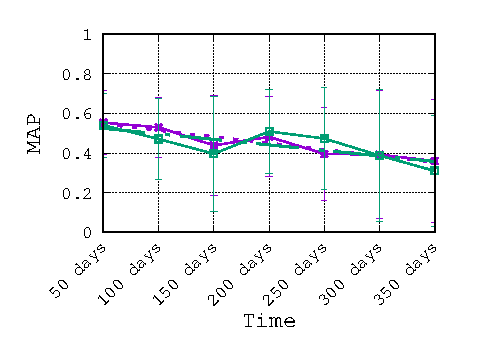
\includegraphics[width=4.9cm]{images/validation_comparaison/average_topics_ap}}
\subfloat[Fig:][]{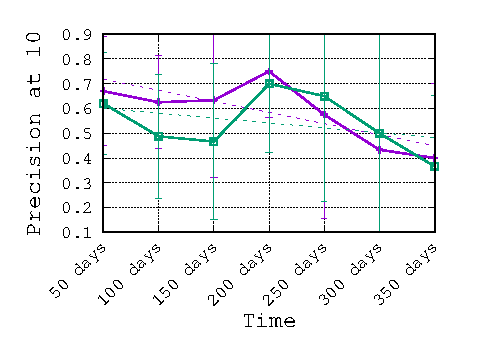
\includegraphics[width=4.9cm]{images/validation_comparaison/average_topics_p10}}
\subfloat[Fig:][]{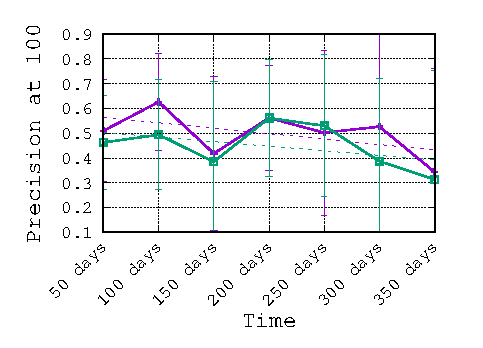
\includegraphics[width=4.9cm]{images/validation_comparaison/average_topics_p100}}
\par\end{centering}
\begin{centering}
\subfloat[Fig:][]{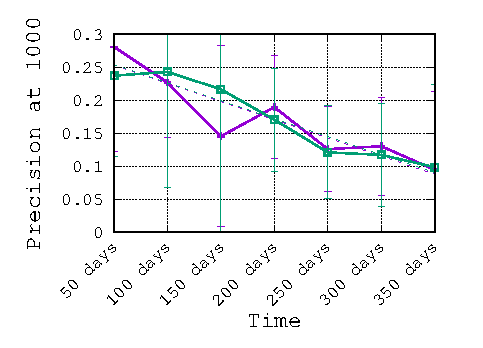
\includegraphics[width=4.9cm]{images/validation_comparaison/average_topics_p1000}}
\subfloat[Fig:][]{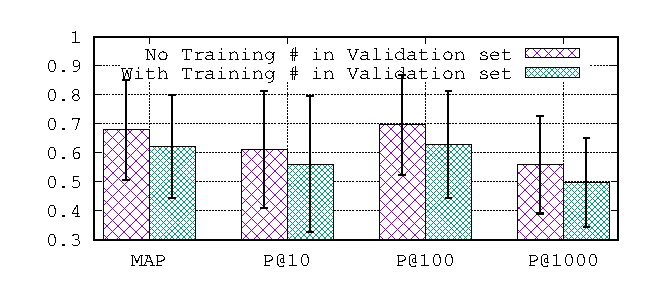
\includegraphics[width=9cm]{images/validation_comparaison/average_topics.eps}}
\par\end{centering}
\caption{Performance obtained while tunning hyperparameters using validation sets with/without tweets containing training hashtags.}
\label{fig:ClassifiersRobustness}
\end{figure}


%Having cases of topical tweets not being correctly labeled as topical,
%provides evidence that our method of labeling tweets has limitations
%and our MAP and P@$n$ values are in fact suffering from this
%problem. However, this shows the power of Logistic Regression method
%in generalizing from a small set of hashtags.




\subsection*{Feature Analysis}
\label{label:featureanalysis}

In this section, we analyze the informativeness of feature sets defined in the Data Description section and the effect of their
attributes on learning targeted topical classifiers. To this end,
our goal in this section is to answer the following questions:
\begin{itemize}
\item What are the best features for learning classifiers and do they differ by topic?
\item For each feature type, do any attributes correlate with importance?
\end{itemize}
To answer these questions, we use Mutual Information (MI)~\cite{manning_ir} as our primary
metric for feature evaluation.  Mutual Information is a general method
for measuring the amount of information one random variable contains
about another random variable and is used to select
predictive features in machine learning.  To calculate the amount of
information that each feature
$j \in \{ \textit{User} \cup \textit{Hashtag} \cup \textit{Mention} \cup \textit{Term} \cup \textit{Location} \}$
provides w.r.t.\ each topic label $t \in \{$Natural Disaster, Epidemics $,\cdots\}$,
Mutual Information is formally defined as:
\begin{align*}
I(j, t) & = \!\!\! \sum_{t \in \{ \mathrm{0}, \mathrm{1} \}} \sum_{j \in \{ \mathrm{0}, \mathrm{1}\}}p(j,t)\log \left ( \frac{p(j,t)}{p(j)p(t)} \right ) 
 \label{eq:eq1}
\end{align*}
with marginal probabilities of topic $p(t)$ and feature $p(j)$ occurrence and joint probability $p(t,j)$ computed over the sample space of all tweets, 
where higher values for this metric indicate more informative features $j$ for the topic $t$.




\begin{figure}[t!]
\centering
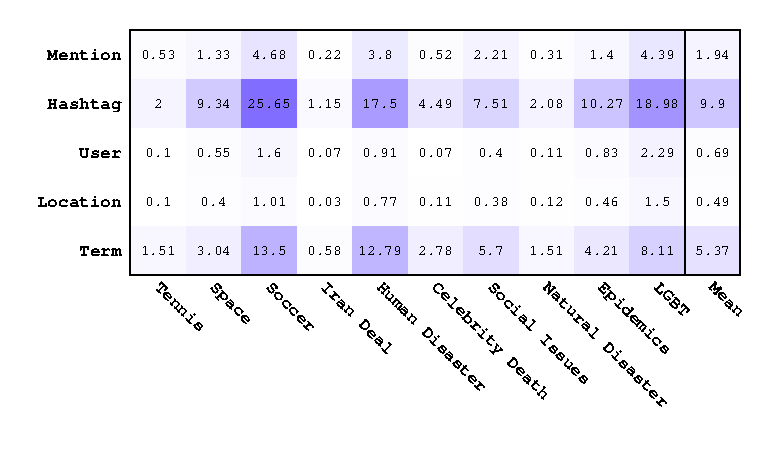
\includegraphics[width=0.75\textwidth]{images/avgMI_gray}%, height=60mm
%\vspace{-3mm}
\caption{Matrix of mean Mutual Information values for different feature types vs. topics.  The last column as average of mean values across all topics.  All values should be multiplied by $10^{-8}$.)}
\label{fig:avgMI}
\end{figure}

\begin{figure*}[tp!]
\centering
\begin{tabular}{ccccc}
%\fbox{\rule{10cm}{3.85cm}}
\subfloat[Fig:][Term.]{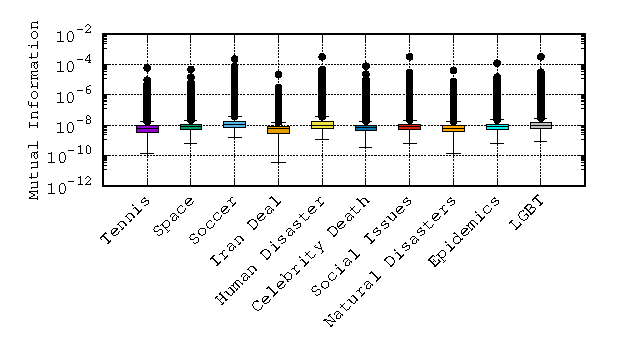
\includegraphics[width=0.34\textwidth]{images/avgMIBoxPlots/term_features}}
\subfloat[Fig:][Location.]{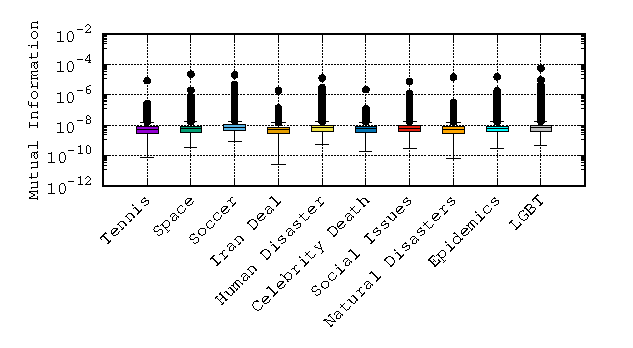
\includegraphics[width=0.34\textwidth]{images/avgMIBoxPlots/loc_features}}
\subfloat[Fig:][Hashtag.]{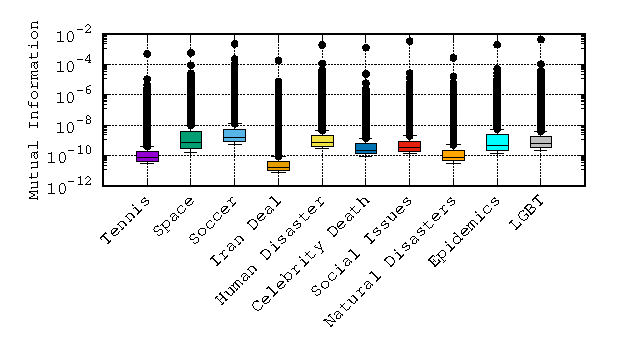
\includegraphics[width=0.34\textwidth]{images/avgMIBoxPlots/hashtag_features}}\\
\subfloat[Fig:][Mention.]{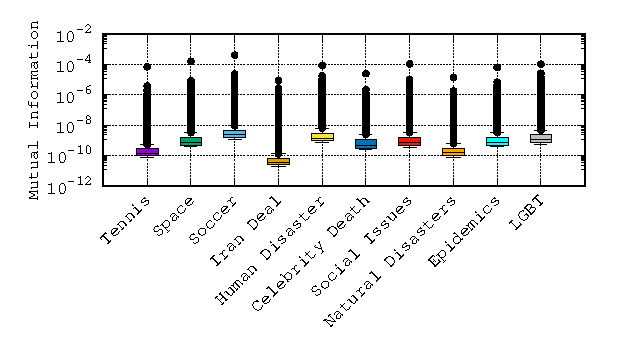
\includegraphics[width=0.33\textwidth]{images/avgMIBoxPlots/mention_features}}
\subfloat[Fig:][User.]{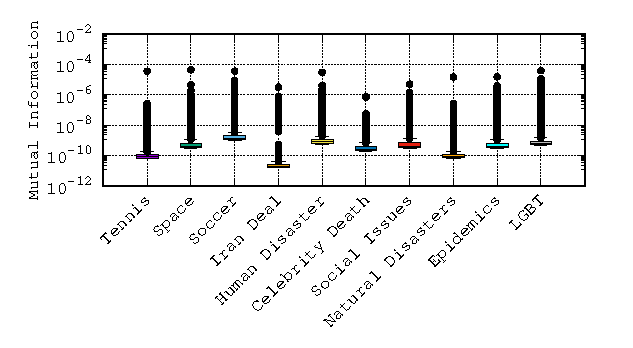
\includegraphics[width=0.33\textwidth]{images/avgMIBoxPlots/user_features}} \\
\end{tabular}
%\vspace{-2mm}
\caption {Box plots of Mutual Information values (y-axis) per feature type across topics (x-axis labels).}
\label{fig:avgMIBP}
\vspace{2mm}
\end{figure*}
%%%%%%%%%%%%%%%%%%%%%%%%%%%%%%%%%%%%%%%%%%%%%%%%%%%%%%%%%%%%%%%%%%%%%%%%%%%
%\vspace*{\floatsep}
%%%%%%%%%%%%%%%%%%%%%%%%%%%%%%%%%%%%%%%%%%%%%%%%%%%%%%%%%%%%%%%%%%%%%%%%%%%

%%%%%%%%%%%%%%%%%%%%%%%%%%%%%%%%%%%%%%%%%%%%%%%%%%%%%%%%%%%%%%%%%%%%%%%%%%%

%%%%%%%%%%%%%%%%%%%%%%%%%%%%%%%%%%%%%%%%%%%%%%%%%%%%%%%%%%%%%%%%%%%%%%%%%%%

%%%%%%%%%%%%%%%%%%%%%%%%%%%%%%%%%%%%%%%%%%%%%%%%%%%%%%%%%%%%%%%%%%



%%%%%%%%%%%%%%%%%%%%%%%%%%%%%%%%%%%%%%%%%%%%%%%%%%%%%%%%%%%%%%%%%%
% \begin{table*}[t!]
% \centering
% \caption{\textcolor{red}{(Zahra):} The top 5 features for each feature type and topic based on Mutual Information.}
% {\renewcommand{\arraystretch}{1.2}
% \resizebox{\textwidth}{!}{%
% \begin{tabular}{|l|l|l|l|l|l|l|l|l|l|l|}
% \hline
% \textbf{Topics/Top10} & \textbf{NaturalDisaster} & \textbf{Epidemics} & \textbf{IranDeal} & \textbf{SocialIssues} & \textbf{LBGT} & \textbf{HumanDisaster} & \textbf{CelebrityDeath} & \textbf{Space} & \textbf{Tennis} & \textbf{Soccer} \\ \hline
% \textbf{From} & earthquake\_wo & changedecopine & mazandara & nsingerdebtpaid & eph4\_15 & ydumozyf & nmandelaquotes & daily\_astrodata & tracktennisnews & losangelessrh \\ \hline
% \textbf{From} & earthalerts & drdaveanddee & hhadi119 & debtadvisoruk & mgdauber & syriatweeten & boiknox & freesolarleads & tennis\_result & shoetale \\ \hline
% \textbf{From} & seelites & joinmentornetwk & 140iran & debt\_protect & stevendickinson & tintin1957 & jacanews & houston\_\_jobs & i\_roger\_federer & sport\_\_agent \\ \hline
% \textbf{From} & globalfloodnews & followebola & setarehgan & negativeequityf & lileensvf1 & sirajsol & ewnreporter & star\_wars\_gifts & tennislessonnow & books\_you\_want \\ \hline
% \textbf{From} & gcmcdrought & localnursejobs & akhgarshabaneh & dolphin\_ls & truckerbooman & rt3syria & paulretweet & lenautilus & kamranisbest & makeupbella \\ \hline \hline
% \textbf{Hashtag} & earthquake & health & iran & ferguson & tcot & syria & rip & science & wimbledon & lfc \\ \hline
% \textbf{Hashtag} & haiyan & uniteblue & irantalks & mikebrown & p2 & gaza & riprobinwilliams & starwars & usopen & worldcup \\ \hline
% \textbf{Hashtag} & storm & ebola & rouhani & ericgarner & pjnet & isis & ripcorymonteith & houston & tennis & arsenal \\ \hline
% \textbf{Hashtag} & tornado & healthcare & iranian & blacklivesmatter & uniteblue & israel & mandela & sun & nadal & worldcup2014 \\ \hline
% \textbf{Hashtag} & prayforthephilippines & depression & no2rouhani & fergusondecision & teaparty & mh370 & nelsonmandela & sxsw & wimbledon2014 & halamadrid \\ \hline \hline
% \textbf{Location} & philippines & usa & tehran & st.louis & usa & malaysia & southafrica & germany & london & liverpool \\ \hline
% \textbf{Location} & ca & ncusa & u.s.a & mo & bordentown & palestine & johannesburg & roodepoort & uk & manchester \\ \hline
% \textbf{Location} & india & garlandtx & nederland & usa & newjersey & syria & capetown & houston & india & london \\ \hline
% \textbf{Location} & newdelhi & oh-sandiego & iran & dc & sweethomealabama! & israel & pretoria & austin & pakistan & nigeria \\ \hline
% \textbf{Location} & newzealand & washington & globalcitizen & washington & aurora & london & durban & tx & islamabad & india \\ \hline \hline
% \textbf{Mention} & oxfamgb & foxtramedia & 4freedominiran & deray & jjauthor & ifalasteen & nelsonmandela & bizarro\_chile & wimbledon & lfc \\ \hline
% \textbf{Mention} & weatherchannel & obi\_obadike & iran\_policy & natedrug & 2anow & revolutionsyria & realpaulwalker & nasa & usopen & arsenal \\ \hline
% \textbf{Mention} & redcross & who & hassanrouhani & antoniofrench & govchristie & drbasselabuward & robinwilliams & j\_ksen & andy\_murray & realmadriden \\ \hline
% \textbf{Mention} & twcbreaking & obadike1 & un & bipartisanism & a5h0ka & mogaza & rememberrobin & jaredleto & serenawilliams & ussoccer \\ \hline
% \textbf{Mention} & abc7 & c25kfree & statedept & theanonmessage & barackobama & palestinianism & tweetlikegiris & 30secondstomars & espntennis & mcfc \\ \hline \hline
% \textbf{Term} & philippines & health & iran & police & obama & israel & robin & cnblue & murray & madrid \\ \hline
% \textbf{Term} & donate & ebola & regime & protesters & gun & gaza & williams & movistar & tennis & goal \\ \hline
% \textbf{Term} & typhoon & acrx & nuclear & officer & rights & israeli & nelson & enero & federer & cup \\ \hline
% \textbf{Term} & affected & medical & iranian & protest & america & killed & mandela & \c{c}imperdible & djokovic & manchester \\ \hline
% \textbf{Term} & relief & virus & resistance & cops & gop & children & cory & greet & nadal & match \\ \hline
% \end{tabular}
% }}
% \end{table*}
%%%%%%%%%%%%%%%%%%%%%%%%%%%%%%%%%%%%%%%%%%%%%%%%%%%%%%%%%%%%%%%%%%

%\textbf{What we have to work with: topics, features, feature attributes}

In order to answer the first question regarding the best features
for learning topical classifiers, we provide the mean Mutual Information
values for each feature across different topics in Figure~\ref{fig:avgMI}.
The last column in Fig.~\ref{fig:avgMI} shows the
average of the mean Mutual Information for each feature type. From analysis of
Figure~\ref{fig:avgMI}, we can make a set of observations:
\begin{itemize}
\item The \textit{Hashtag} and \textit{Term} features are the most informative features on average. \textcolor{red}{ \textit{Hashtags} are commonly used on Twitter to tag topics of interest associated with a given post, which explains their high informativness.}

% and in general, the more features you have, the better the chance that one is useful.
\item \textcolor{red}{The topics \textit{Iran Deal}, \textit{Tennis} and \textit{Natural Disasters} have low overal features correlation based on Mutual Information. However, these topics  are in the list of top MAP scores using the \textit{Logistic Regression} classifier.}

\item The Location feature provides the highest MI regarding the topics of \textit{Human Disaster}, \textit{LBGT}, and \textit{Soccer} indicating a lot of content in these topics is heavily localized.
\item \textcolor{red}{ Looking at the overall average values, the order of informativeness of feature types appears to be the following: \textit{Hashtag}, \textit{Term}, \textit{Mention}, \textit{User}, \textit{Location}.}
\end{itemize}
To further analyze the relationship between the informativeness of feature types and topics,
we refer to the box plots of Figure~\ref{fig:avgMIBP}.  Here we see the quartiles and outliers of
the distribution rather than just the average of the MI values in order to ensure the mean MI
values were not misleading our interpretations.  Overall, the story is the same: \textcolor{red}{ hashtag
and term} features dominate in terms of MI followed by the other less informative
features.  Furthermore, two observations are apparent: (1) hashtags have more outliers indicating that
\emph{the most useful individual features may be terms}, and (2) the topic has little impact on which feature
is most important indicating \emph{stability of feature type informativeness over topics}.

As anecdotal evidence to inspect which features are most informative, we refer to
Table~\ref{table:top10MItopicsLocations}, which displays the top five feature instances
for each feature type and topic. \textcolor{red}{For example the term \textit{typhoon} is the most correlated feature term with the topic \textit{Natural Disaster}, the official \textit{UNICEF}\footnote{The United Nations Children's Fund (UNICEF) is an organization that aims to provide emergency food and healthcare to children and mothers in developing countries everywhere.} twitter account (\textit{@unicef}) is the most correlated feature mention with the Human Disaster topic, and the hashtag \textit{\#science} is the most correlated hashtag feature with the topic \textit{Space}.}
Among many remarkable insights in this table, one key aspect  
we note is that the \emph{terms appear to be the most generic} (and hence most generalizable) features,
providing strong intuition as to why these features figure so prominently in terms of
their informativeness.  The top \emph{locations are also highly relevant to most topics} indicating
the overall importance of these tweet features for identifying topical tweets.

\begin{table*}[t!]
\centering
\caption{ The top 5 features for each feature type and topic based on Mutual Information.}
{\renewcommand{\arraystretch}{1.2}
\resizebox{\textwidth}{!}{%
\begin{tabular}{|l|l|l|l|l|l|l|l|l|l|l|}
\hline 
\textbf{Topics/Top10} & \textbf{Natural Disaster} & \textbf{Epidemics} & \textbf{Iran Deal} & \textbf{Social Issues} & \textbf{LBGT} & \textbf{Human Disaster} & \textbf{Celebrity Death} & \textbf{Space} & \textbf{Tennis} & \textbf{Soccer}\tabularnewline
\hline 
\hline 
\textbf{User} & from\_japan & changedecopine & mazandara & debtadvisoruk & stevendickinson & witfp & boiknox & daily\_astrodata & tracktennisnews & makeupbella\tabularnewline
\hline 
\textbf{User} & everyearthquake & stylishoz & freeiran9292 & nsingerdebtpaid & mgdauber & ydumozyf & jacanews & freesolarleads & novakdjokovic\_i & sport\_agent\tabularnewline
\hline 
\textbf{User} & quakestoday & drdaveanddee & hhadi119 & negativeequityf & lileensvf1 & syriatweeten & ewnreporter & sciencewatchout & i\_roger\_federer & yasmingoode\tabularnewline
\hline 
\textbf{User} & equakea & soliant\_schools & balouchn2 & iris\_messenger & kevinwhipp & rk70534 & rowwsupporter & houston\_jobs & andymurrayfans1 & sportsroadhouse\tabularnewline
\hline 
\textbf{User} & davewinfields & msgubot & jeffandsimon & dolphin\_ls & petermabraham & gosyrianews & flykiidchris & lenautilus & rafaelnadal\_fan & losangelessrh\tabularnewline
\hline 
\hline 
\textbf{Hashtag} & \#earthquake & \#health & \#iran & \#ferguson & \#tcot & \#syria & \#rip & \#science & \#wimbledon & \#worldcup\tabularnewline
\hline 
\textbf{Hashtag} & \#haiyan & \#uniteblue & \#irantalks & \#mikebrown & \#pjnet & \#gaza & \#ripcorymonteith & \#sun & \#tennis & \#lfc\tabularnewline
\hline 
\textbf{Hashtag} & \#storm & \#ebola & \#iranian & \#ericgarner & \#p2 & \#israel & \#riprobinwilliams & \#houston & \#usopen & \#football\tabularnewline
\hline 
\textbf{Hashtag} & \#PrayForThePhilippines & \#healthcare & \#rouhani & \#blacklivesmatter & \#uniteblue & \#gazaunderattack & \#rippaulwalker & \#starwars & \#nadal & \#worldcup2014\tabularnewline
\hline 
\textbf{Hashtag} & \#tornado & \#fitness & \#irantalksvienna & \#icantbreathe & \#teaparty & \#isis & \#robinwilliams & \#scifi & \#wimbledon2014 & \#sports\tabularnewline
\hline 
\hline 
\textbf{Location} & With everyone & USA & France & St Louis MO & USA & Syria & South Africa & Houston TX & Worldwide & Liverpool\tabularnewline
\hline 
\textbf{Location} & Earth & Francophone & Tehran Iran & Washington DC & Bordentown New Jersey & Palestine & Pandaquotescom & Germany & London & Manchester\tabularnewline
\hline 
\textbf{Location} & Philippines & United States & Inside of Iran & St Louis & Global Markets & Syrian Arab Republic & Johannesburg South Africa & Houston & The Midlands & London\tabularnewline
\hline 
\textbf{Location} & Don't follow me am i a bot & Gainesville FL USA & Iran & Virginia US & The blue regime of Maryland & Israel & Johannesburg & Rimouski & London UK & Anfield\tabularnewline
\hline 
\textbf{Location} & Global planet earth & Boulder Colorado & Washington DC & Saint Louis MO & Lancaster county PA & Washington DC & Cape Town & In a galaxy far far ebay & Wimbledon & Bangil East Java Indonesia\tabularnewline
\hline 
\hline 
\textbf{Mention} & @oxfamgb & @foxtramedia & @ap & @natedrug & @jjauthor & @ifalasteen & @nelsonmandela & @nasa & @wimbledon & @lfc\tabularnewline
\hline 
\textbf{Mention} & @gabriele\_corno & @obi\_obadike & @afp & @deray & @2anow & @drbasselabuward & @realpaulwalker & @philae2014 & @usopen & @fifaworldcup\tabularnewline
\hline 
\textbf{Mention} & @weatherchannel & @who & @iran\_policy & @antoniofrench & @gop & @revolutionsyria & @ddlovato & @maximaxoo & @atpworldtour & @ussoccer\tabularnewline
\hline 
\textbf{Mention} & @twcbreaking & @kayla\_itsines & @4freedominiran & @bipartisanism & @pjnet\_blog & @unicef & @robinwilliams & @esa\_rosetta & @andy\_murray & @mcfc\tabularnewline
\hline 
\textbf{Mention} & @redcross & @canproveit & @orgiac & @theanonmessage & @espuelasvox & @free\_media\_hub & @historicalpics & @astro\_reid & @wta & @realmadriden\tabularnewline
\hline 
\hline 
\textbf{Term} & typhoon & health & nuclear & police & obama & israeli & robin & space & tennis & liverpool\tabularnewline
\hline 
\textbf{Term} & philippines & ebola & regime & protesters & gun & israel & williams & solar & murray & cup\tabularnewline
\hline 
\textbf{Term} & magnitude & outbreak & iran & officer & america & gaza & walker & moon & djokovic & supporting\tabularnewline
\hline 
\textbf{Term} & storm & virus & iranian  & cops & obamacare & palestinian & cory & houston & federer & match\tabularnewline
\hline 
\textbf{Term} & usgs & acrx & mullahs & protest & gop & killed & paul & star & nadal & goal\tabularnewline
\hline 
\end{tabular}

}}
\label{table:top10MItopicsLocations}
\end{table*}







% Need more insight than this! -SPS
%
%It can be observed that the different locations, hashtags, or terms
%shown as the top features based on Mutual Information are actually in
%relation with the specific topic.

In order to answer the second question on whether any attributes
correlate with importance for each feature, we provide two types of
analysis \textcolor{red}{using the topic \textit{Celebrity Death} -- 
the other topics showed similar patterns, thus we have chosen to omit them.} 
The first analysis shown in Figure~\ref{fig:violinplots}
analyzes the distributions of Mutual Information values for features
when binned by the magnitude of various attributes of those
features, outlined as follows:
\begin{itemize}
\item \textbf{From} vs. 
\begin{itemize}
\item \textit{Favorite count:} \# of tweets user has favorited.
\item \textit{Followers count:} \# of users who follow user.
\item \textit{Friends count:} \# of users followed by user.
\item \textit{Hashtag count:} \# of hashtags used by user.
\item \textit{Tweet count:} \# of tweets from user.
 \end{itemize}
\end{itemize}
\begin{itemize}
\item \textbf{Hashtag} vs.
\begin{itemize}
\item \textit{Tweet count:} \# of tweets using hashtag.
\item \textit{User count:} \# of users using hashtag.
\end{itemize}
\end{itemize}
\begin{itemize}
\item \textbf{Location} vs. \textit{User count:} \# of users using location.
\item \textbf{Mention} vs. \textit{Tweet count:} \# of tweets using mention.
\item \textbf{Term} vs. \textit{Tweet count:} \# of tweets using term.
\end{itemize}

As we can see in the boxplots of Figure~\ref{fig:violinplots}, the
general pattern is that the greater the number of tweets, users, or
hashtag count a feature has, the more informative the feature is in general.
This pattern also exists to some extent on the attributes
of the \textit{From} feature, although the pattern is less visible in
general and not clear (or very weak) for the follower or friend count.
In general, the informativeness of a user appears to have little correlation
with their follower or friend count.

\textcolor{red}{Figure~\ref{fig:densityplots} provides a further analysis by showing
density plots of the tweet count attribute  of the \textit{User}, \textit{Hashtag},
\textit{Mention} and \textit{Term}  features, and the user count attribute of 
the \textit{Hashtag} feature. Here we can clearly observe the positive linear correlation
that exists between the attribute magnitude and the Mutual Information value.
}
%Here we see an
%interesting phenomenon that was not clear in the Violin plots: there
%is a very clear bimodality of the density.  On further investigation
%it turns out that the top mode feature occurs in at least one topical
%tweet whereas the bottom mode occurs in no topical tweets.  While the
%bottom mode features may serve as good indicators of non-topicality,
%the top mode are inherently more indicative of topicality, which
%justifies feature selection by mutual information.



\begin{figure*}[tp!]
\centering
\begin{tabular}{ccccc}
\begin{tabular}{ccccc} % height=35mm -- always scale graphics proportionally by just specifying one dim. -SPS
\subfloat[Fig:][ User \# of favorites.]{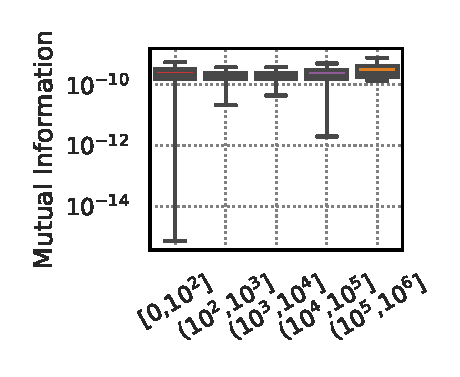
\includegraphics[width=0.19\textwidth]{images/BoxPlots_Cele_death/Cele_death_user_favouritesCount_boxplots.eps}}
\subfloat[Fig:][User \# of followers.]{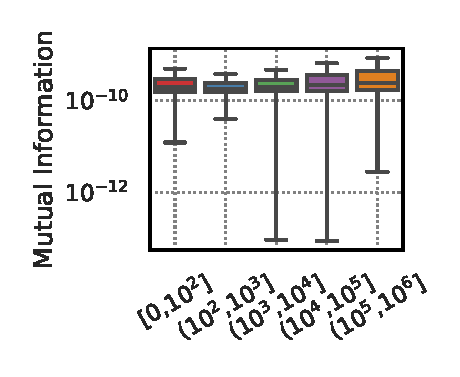
\includegraphics[width=0.19\textwidth]{images/BoxPlots_Cele_death/Cele_death_user_followersCount_boxplots.eps}}
\subfloat[Fig:][User \# of friends.]{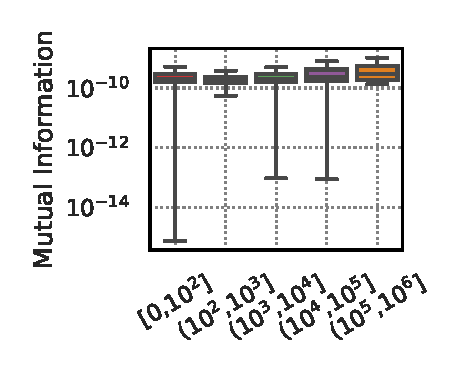
\includegraphics[width=0.19\textwidth]{images/BoxPlots_Cele_death/Cele_death_user_friendsCount_boxplots.eps}}
\subfloat[Fig:][User \# of hashtags.]{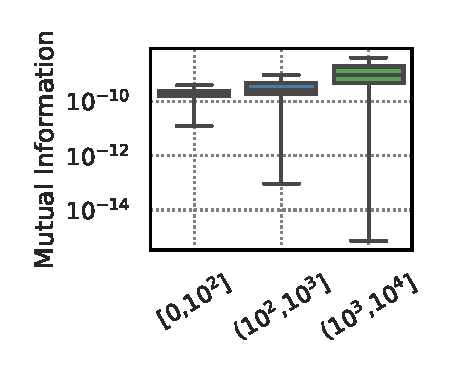
\includegraphics[width=0.19\textwidth]{images/BoxPlots_Cele_death/Cele_death_user_hashtagCount_boxplots.eps}}
\subfloat[Fig:][User \# of tweets.]{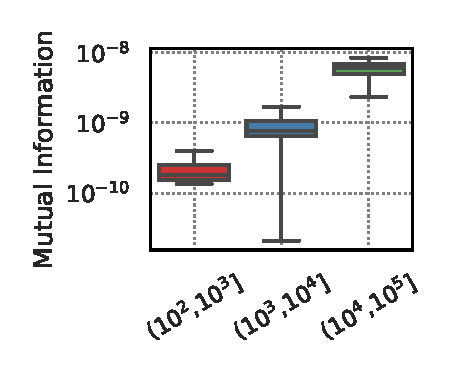
\includegraphics[width=0.19\textwidth]{images/BoxPlots_Cele_death/Cele_death_user_tweetCount_boxplots.eps}} \\
%\vspace{-10mm}
\subfloat[Fig:][Hashtag \# of tweets.]{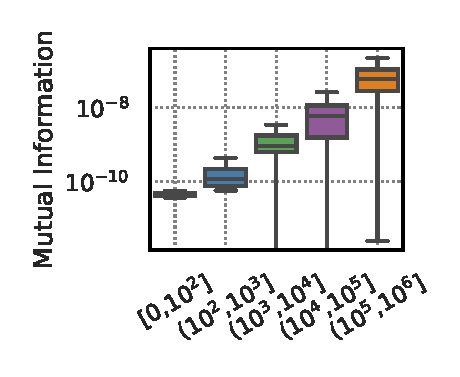
\includegraphics[width=0.19\textwidth]{images/BoxPlots_Cele_death/Cele_death_hashtag_tweetCount_boxplots.eps}}
\subfloat[Fig:][Hashtag \# of users.]{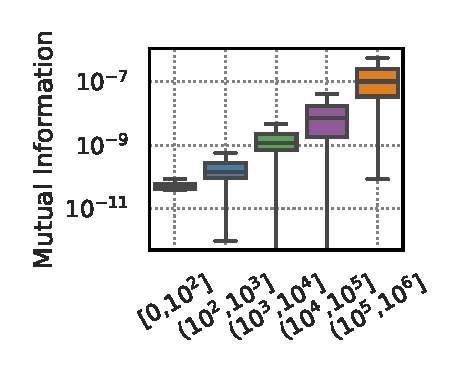
\includegraphics[width=0.19\textwidth]{images/BoxPlots_Cele_death/Cele_death_hashtag_userCount_boxplots.eps}}
\subfloat[Fig:][Location \# of users.]{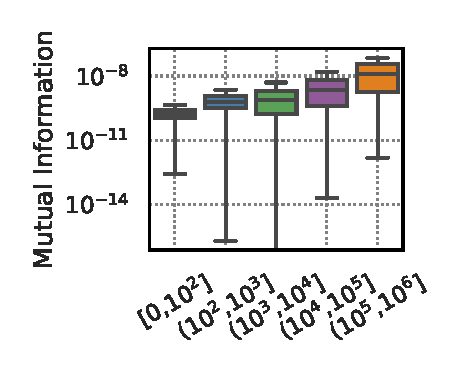
\includegraphics[width=0.19\textwidth]{images/BoxPlots_Cele_death/Cele_death_location_userCount_boxplots.eps}}
\subfloat[Fig:][Mention \# of tweets.]{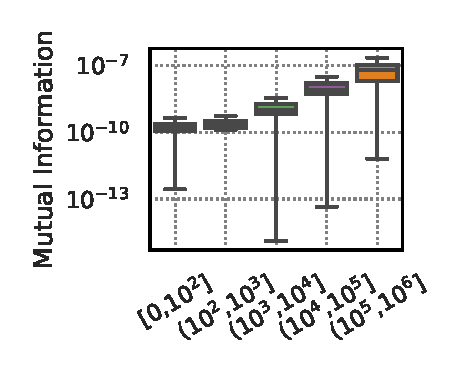
\includegraphics[width=0.19\textwidth]{images/BoxPlots_Cele_death/Cele_death_mention_tweetCount_boxplots.eps}}
\subfloat[Fig:][Term \# of tweets.]{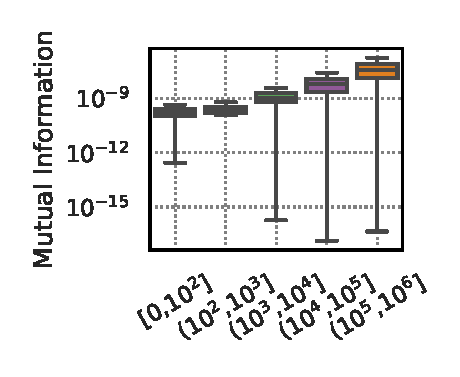
\includegraphics[width=0.19\textwidth]{images/BoxPlots_Cele_death/Cele_death_term_tweetCount_boxplots.eps}} \\
\end{tabular}
\end{tabular}
%\vspace{-2mm}
\caption {Boxplots for the distribution of Mutual Information values (y-axis) of different features as a function of their attribute values (binned on x-axis).  Plots (a-e) respectively show attributes \{favoriteCount, followerCount, friendCount, hashtagCount, tweetCount\} for \textit{From} feature. Plots (f-j) respectively show attributes tweetCount and userCount for \textit{Hashtag}, userCount for \textit{Location} feature, tweetCount for \textit{Mention} and \textit{Term} features.}
\label{fig:violinplots}
\vspace{2mm}
\end{figure*}

\begin{figure*}[t!]
\centering
\begin{tabular}{cccc} % height=35mm -- always scale graphics proportionally by just specifying one dim. -SPS
\subfloat[Fig:][]{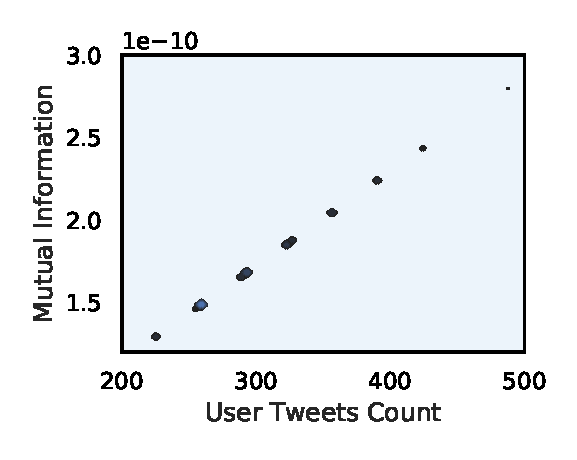
\includegraphics[width=2.6cm]{images/DensityPlots_Cele_death/Cele_death_user_tweetCount_scatter.eps}}
\subfloat[Fig:][]{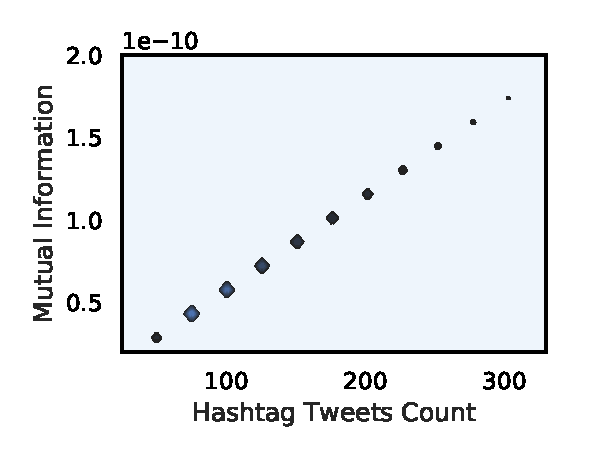
\includegraphics[width=2.6cm]{images/DensityPlots_Cele_death/Cele_death_hashtag_tweetCount_scatter.eps}} \quad
\subfloat[Fig:][]{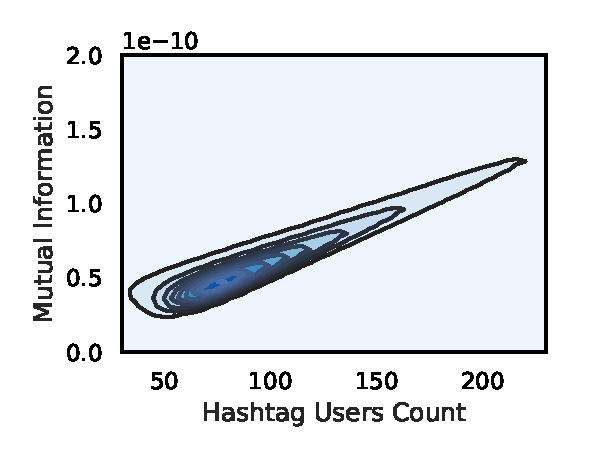
\includegraphics[width=2.6cm]{images/DensityPlots_Cele_death/Cele_death_hashtag_userCount_scatter.eps}} \quad
\subfloat[Fig:][]{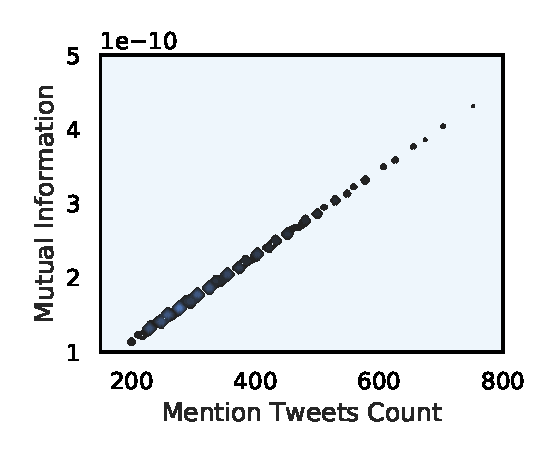
\includegraphics[width=2.6cm]{images/DensityPlots_Cele_death/Cele_death_mention_tweetCount_scatter.eps}} \quad
\subfloat[Fig:][]{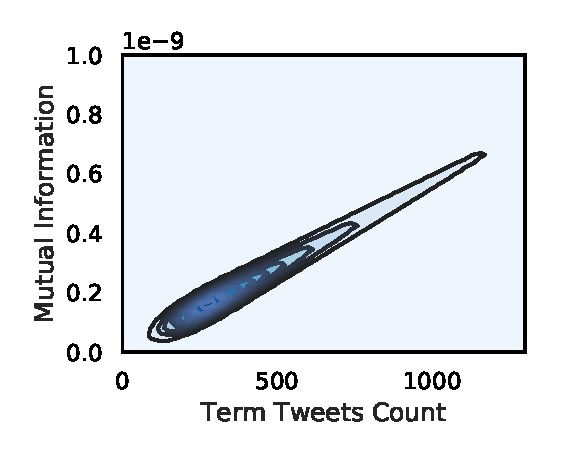
\includegraphics[width=2.6cm]{images/DensityPlots_Cele_death/Cele_death_term_tweetCount_scatter.eps}}\quad
\end{tabular}
\vspace{-2mm}
\caption {Density plots for the frequency values of feature attributes (x-axis) vs. Mutual Information (y-axis).  Plots (a-d) respectively show attributes \{favoriteCount, followerCount, friendCount, hashtagCount\} for the \textit{From} feature.}
\label{fig:densityplots}
\vspace{2mm}
\end{figure*}
